\chapter{Proof-of-Concept Applicatie}
\label{ch:ontwikkeling}

\section{Inleiding}

Dit hoofdstuk dient als een uitgebreide toelichting op de softwareoplossing die binnen deze bachelorproef is ontwikkeld.
Eerst zullen de verschillende componenten van de applicatie worden besproken, gevolgd door een gedetailleerde uitleg over hoe een gebruiker de applicatie kan gebruiken.
Aangezien er rekening gehouden werd met het effectief inzetten van de applicatie in de praktijk, zullen ook de gebruikte technologieën en technische keuzes worden toegelicht.
Zo kan de software bij opeenvolgende bachelorproeven iteratief verder ontwikkeld worden voor nieuwe toepassingen en verbeteringen.

\section{Applicatiecomponenten en Gebruikersinteractie}

De workflow die bedacht werd voor de proof-of-concept applicatie, om van ruwe data naar bruikbare metrieken te gaan, kan als volgt worden samengevat:
\begin{enumerate}
    \item Er worden één of meerdere `kalibratie-opnames' gemaakt met de eyetrackingbril, waarbij elk object dat onderdeel is van het onderzoek, vanuit verschillende hoeken wordt gefilmd.
    \item Ook worden er opnames gemaakt die daarna geanalyseerd worden, waarbij de studenten in de simulatieomgeving met de eyetrackingbril rondlopen.
    \item De opnames worden geïmporteerd in de applicatie via de WiFi-verbinding van de eyetrackingbril.
    \item Men geeft een naam aan de simulatieomgeving (bijvoorbeeld `Zorglab Zorgkamer') binnen de applicatie en defininieert de objecten.
    \item Daarna kan men beginnen met het labelen van de objecten in de kalibratie-opnames via de ingebouwde labeling-tool. De labeling-data dient als een basis voor het trainen of initialiseren van de analysemodellen.
    \item De applicatie is nu in staat de eyetracking-opnames van de studenten te analyseren en de metrieken te visualiseren. Het visualisatiegedeelte werd niet verder uitgewerkt binnen deze bachelorproef omdat er geen betrouwbaar analysemodel kon worden bekomen; maar verder hierover in Hoofdstuk~\ref{ch:experiment}.
\end{enumerate}
De applicatie is dus opgebouwd uit verschillende componenten die samen een stapsgewijs proces vormen. Deze zullen hieronder verder worden toegelicht.

\subsubsection{Opnames Maken}

Voordat de applicatie ontwikkeld kon worden, waren er eerst een aantal video-opnames nodig. 
In deze fase werd de Tobii eyetracking-bril van het Zorglab ontleend om vertrouwd te raken met het maken van opnames. 
Deze opnames werden thuis uitgevoerd en dienden zowel als basis voor de applicatie zelf als voor initiële experimenten met de computer vision-modellen die later zouden worden ingezet in de labelingtool en de analyses.
Om een opname te maken hebben we twee zaken nodig: de eyetracker zelf met bijbehorende accessoires, en een laptop of computer waarop de `Tobii Pro Glasses 3 Controller'\footnote{\url{https://www.tobii.com/products/eye-trackers/wearables/tobii-pro-glasses-3/controller-app}} app is geïnstalleerd.

\begin{figure}[H]
  \centering
  
\includegraphics[width=0.6\textwidth]{placeholder.jpeg}
  \caption[]{\label{fig:todo} TODO: Foto met de benodigdheden: eyetracker, hub, laptop met app zichtbaar (eyetracker niet geconnecteerd), batterijlader, kalibratiekaart
 }
\end{figure}

De eyetracker zelf bestaat uit een hub die stroom levert aan de bril en de opnames opslaat op een SD-kaart. Daarnaast is er de bril zelf die op het hoofd van de gebruiker wordt geplaatst.
De hub heeft een batterij die opgeladen kan worden met de bijgeleverde oplader. 
Eens de bril geconnecteerd is met de hub via de ingebouwde HDMI-kabel en de hub aan staat met een groen LED-lampje, zou er een WiFi-verbinding moeten verschijnen op de laptop of computer.
Deze verbinding start met `TG', gevolgd door het serienummer van de bril. Het wachtwoord voor de verbinding is `TobiiGlasses'. 
Open de Tobii Pro Glasses 3 Controller-app en observeer of het camerabeeld van de bril zichtbaar is in de app.

\begin{figure}[H]
  \centering
  
\includegraphics[width=0.6\textwidth]{placeholder.jpeg}
  \caption[]{\label{fig:todo} TODO: Foto van de app met camerabeeld zichtbaar, en de knoppen om opnames te maken
 }
\end{figure}

Na het invoegen van de naam van de opname (of participant), druk op de knop `Record' om de opname te starten.
Voordat de opname kan starten, zal de app vragen om de bril te kalibreren. 
Dit kan gedaan worden met de bijgeleverde kalibratiekaart, die op armlengte afstand van de bril dient gehouden te worden.
Aan de participant wordt gevraagd om naar de centrale stip op de kaart te kijken, en vervolgens wordt er op de knop `Calibrate' gedrukt.
De app zal nu beginnen met het opnemen van de video, en de participant kan nu vrij rondlopen in de simulatieomgeving.

% TODO: Best-practices toevoegen?

\subsubsection{Importeren van Eyetracking-Opnames}

Zoals eerder vermeld heeft de Tobii eyetracker twee componenten: de bril zelf en een `hub' die stroom levert aan de bril en de opnames opslaat op een SD-kaart.
Het zou dus mogelijk zijn om de opnames via de SD-kaart te importeren, maar dit is niet praktisch omdat de SD-kaart steeds uit de hub dient gehaald te worden.
Daarom biedt de hub ook een WiFi-verbinding aan, zodat de opnames via een netwerkverbinding kunnen worden geïmporteerd. 

Wanneer men de proof-of-concept applicatie opent op de pagina `Browse Recordings' via de navigatiekolom, worden er twee tabellen getoond (zie figuur \ref{fig:browse-recordings})

\begin{figure}[H]
  \centering
  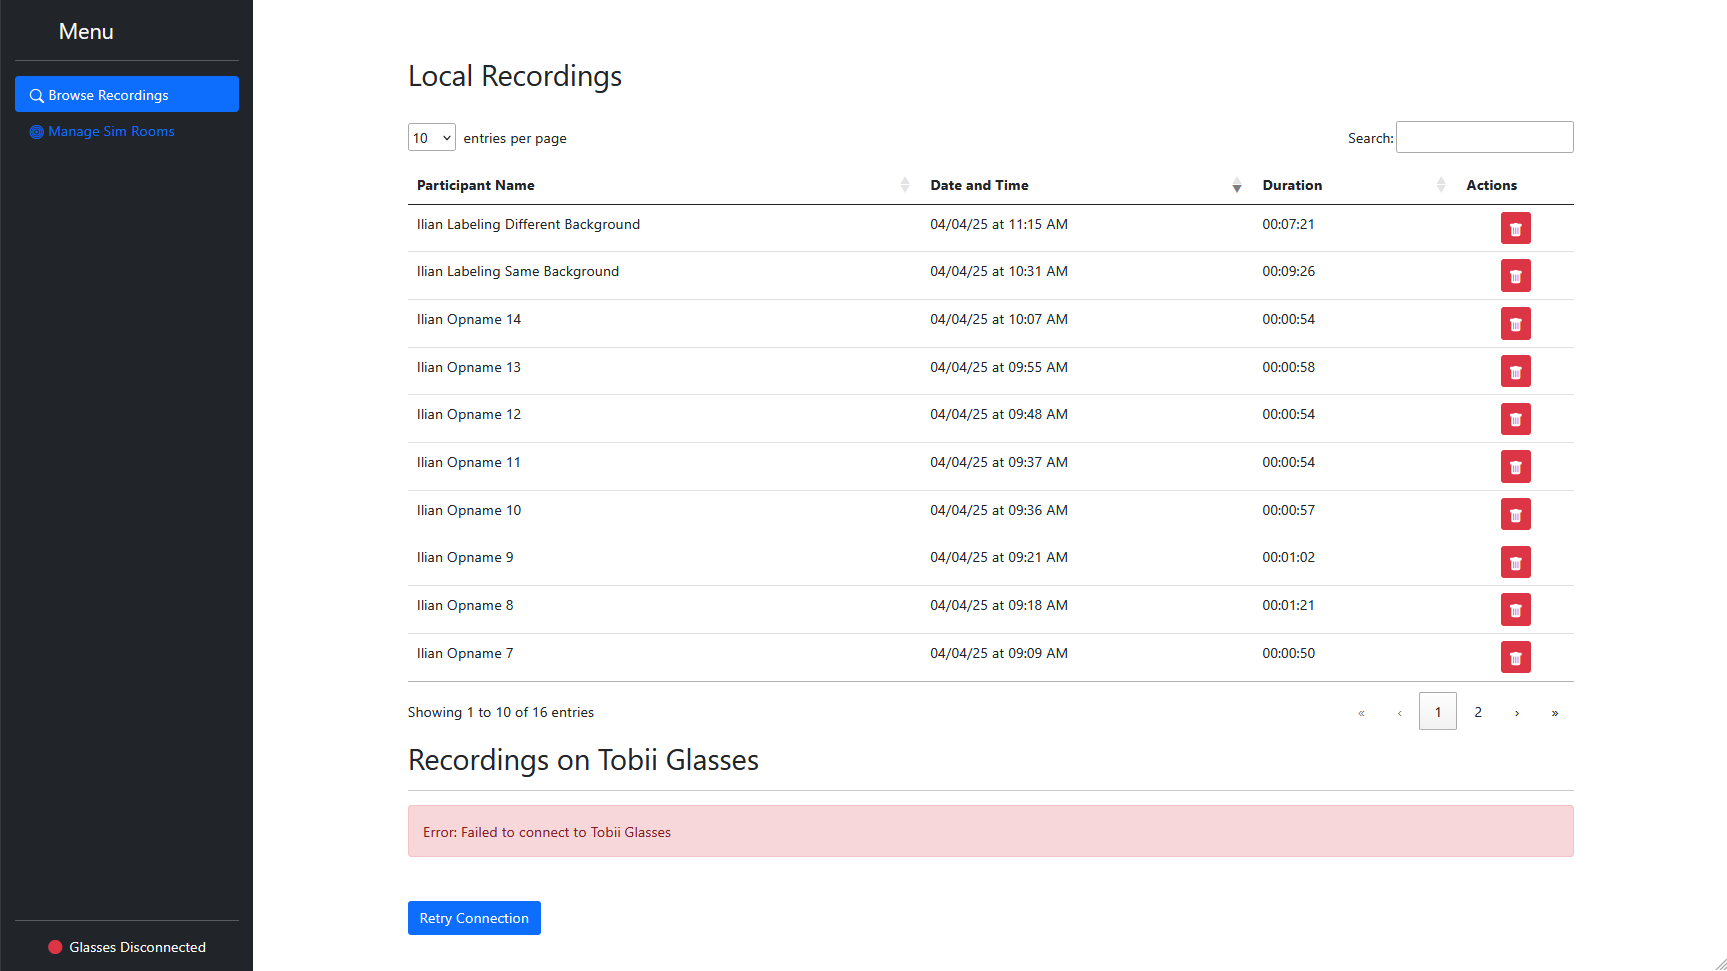
\includegraphics[width=1\textwidth]{browse-recordings.png}
  \caption[]{\label{fig:browse-recordings} Screenshot van de `Browse Recordings'-pagina waar opnames kunnen worden geïmporteerd. Hier is de bril niet verbonden met de computer. }
\end{figure}


De bovenstaande tabel `Local Recordings' toont de opnames die lokaal zijn opgeslagen op de computer, en de onderste tabel `Recordings on Tobii Glasses' toont de opnames die zijn opgeslagen op de hub.
Indien een tabel geen opnames bevat, wordt er een passend bericht getoond.
De opnames worden getoond in tabellen met de naam van elke opname, de datum en tijd waarop deze werd gemaakt, evenals de duur van de opname. 
Het is mogelijk om opnames te verwijderen uit de `Local Recordings'-tabel door op de rode knop met het prullenbakje te klikken naast een opname. Dit heeft geen invloed op de opnames die zijn opgeslagen op de hub.
Ook kan men zoeken naar opnames via de zoekbalk bovenaan de tabellen, en kan men ze sorteren op naam, datum of duur door op de bijbehorende kolomkop te klikken.

Wanneer de bril niet verbonden is met de computer, wordt er een aangepaste melding getoond, met een knop om opnieuw te verbinden. Figuur \ref{fig:browse-recordings} toont een voorbeeld van de interface van de applicatie, waar de bril niet verbonden is met de computer.
Linksonder in de interface toont de applicatie de huidige status van de verbinding met de bril, inclusief de batterijstatus. Bij figuur \ref{fig:browse-recordings-connected} is de bril wel verbonden met de computer. 
Elke rij in de onderste tabel bevat een blauwe knop met een pijl naar beneden, waarmee een opname kan worden geïmporteerd vanuit de bril naar de computer. Dit kan enige tijd duren, afhankelijk van de grootte van de opname.

\begin{figure}[H]
  \centering
  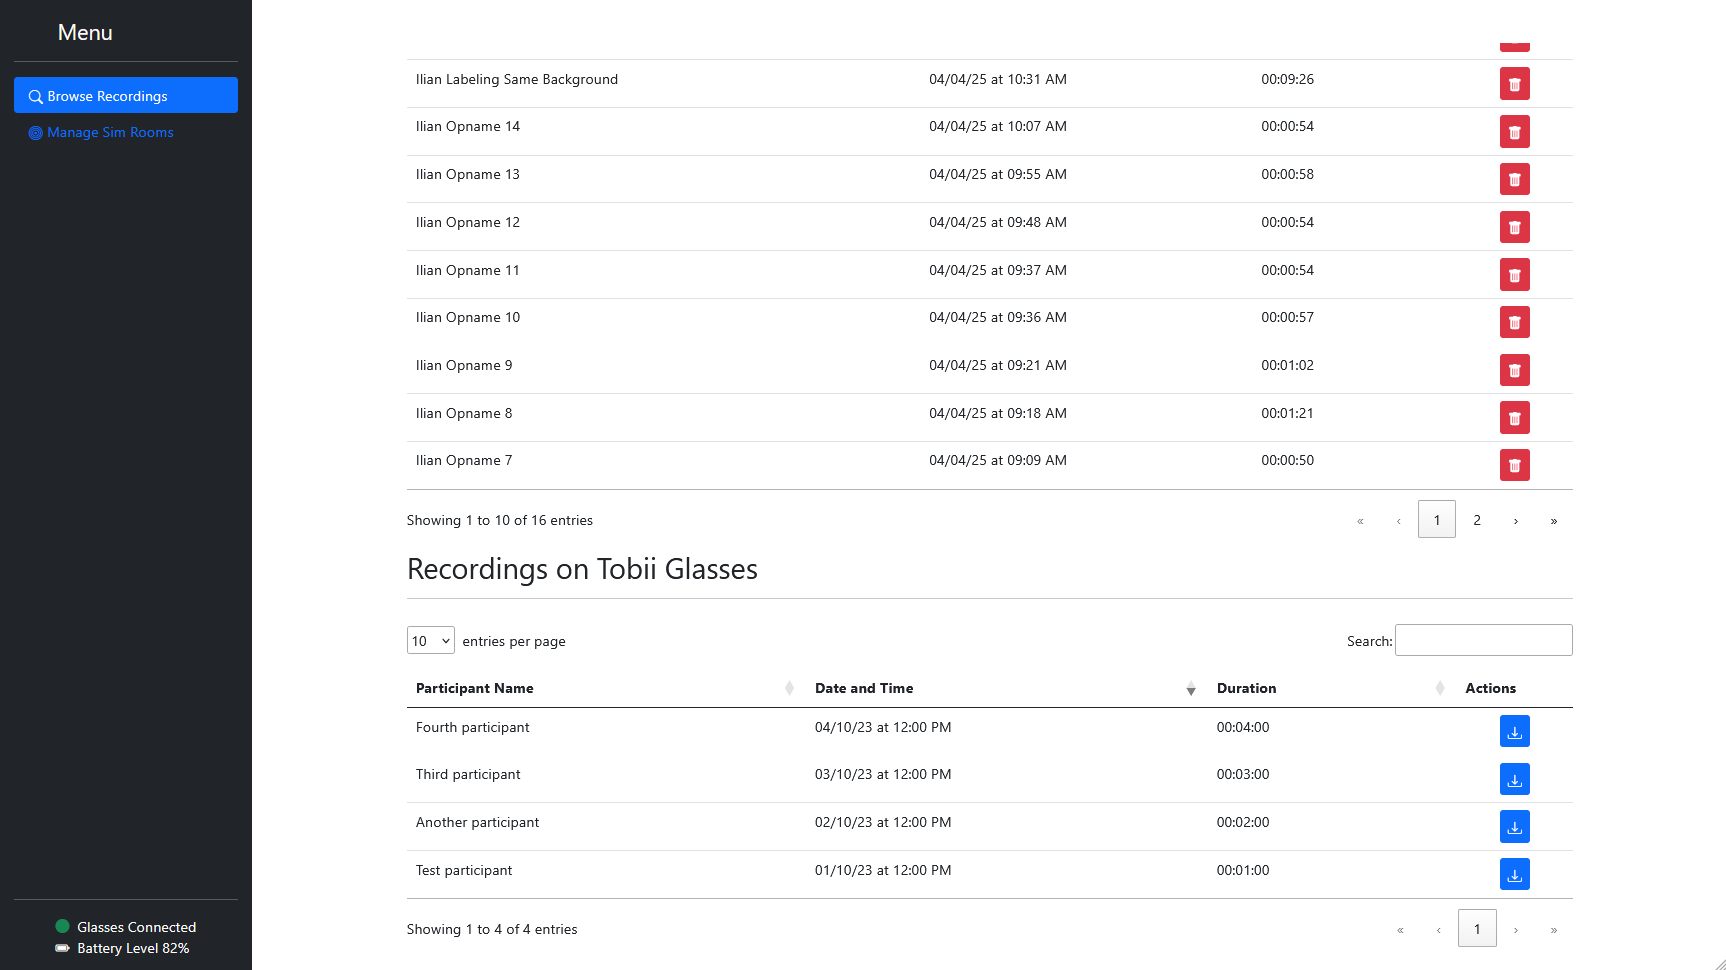
\includegraphics[width=1\textwidth]{browse-recordings-connected.png}
  \caption[]{\label{fig:browse-recordings-connected} Bij dit voorbeeld is de bril wel verbonden met de computer. Men ziet linksonder de batterlijstatus van de bril. In de onderste tabel is het mogelijk om opnames te importeren vanuit de bril naar de computer. }
\end{figure}

\subsubsection{Simulatieruimten en Objecten}

Eens de opnames zijn geïmporteerd, kunnen we overgaan tot het definiëren van de objecten in de kalibratie-opnames. Één van de design-keuzes was om met zogenaamde `simulatieruimten` te werken die verschillende omgevingen voorstellen, elk met hun eigen objecten.
Men kan zich dus voorstellen dat men niet enkel in het Zorglab werkt, maar bijvoorbeeld ook in een echt ziekenhuis of een woonzorgcentrum. Het doel was dus om de applicatie zo gebruiksvriendelijk mogelijk te maken, om het werk van de trainers te vergemakkelijken.

\begin{figure}[H]
  \centering
  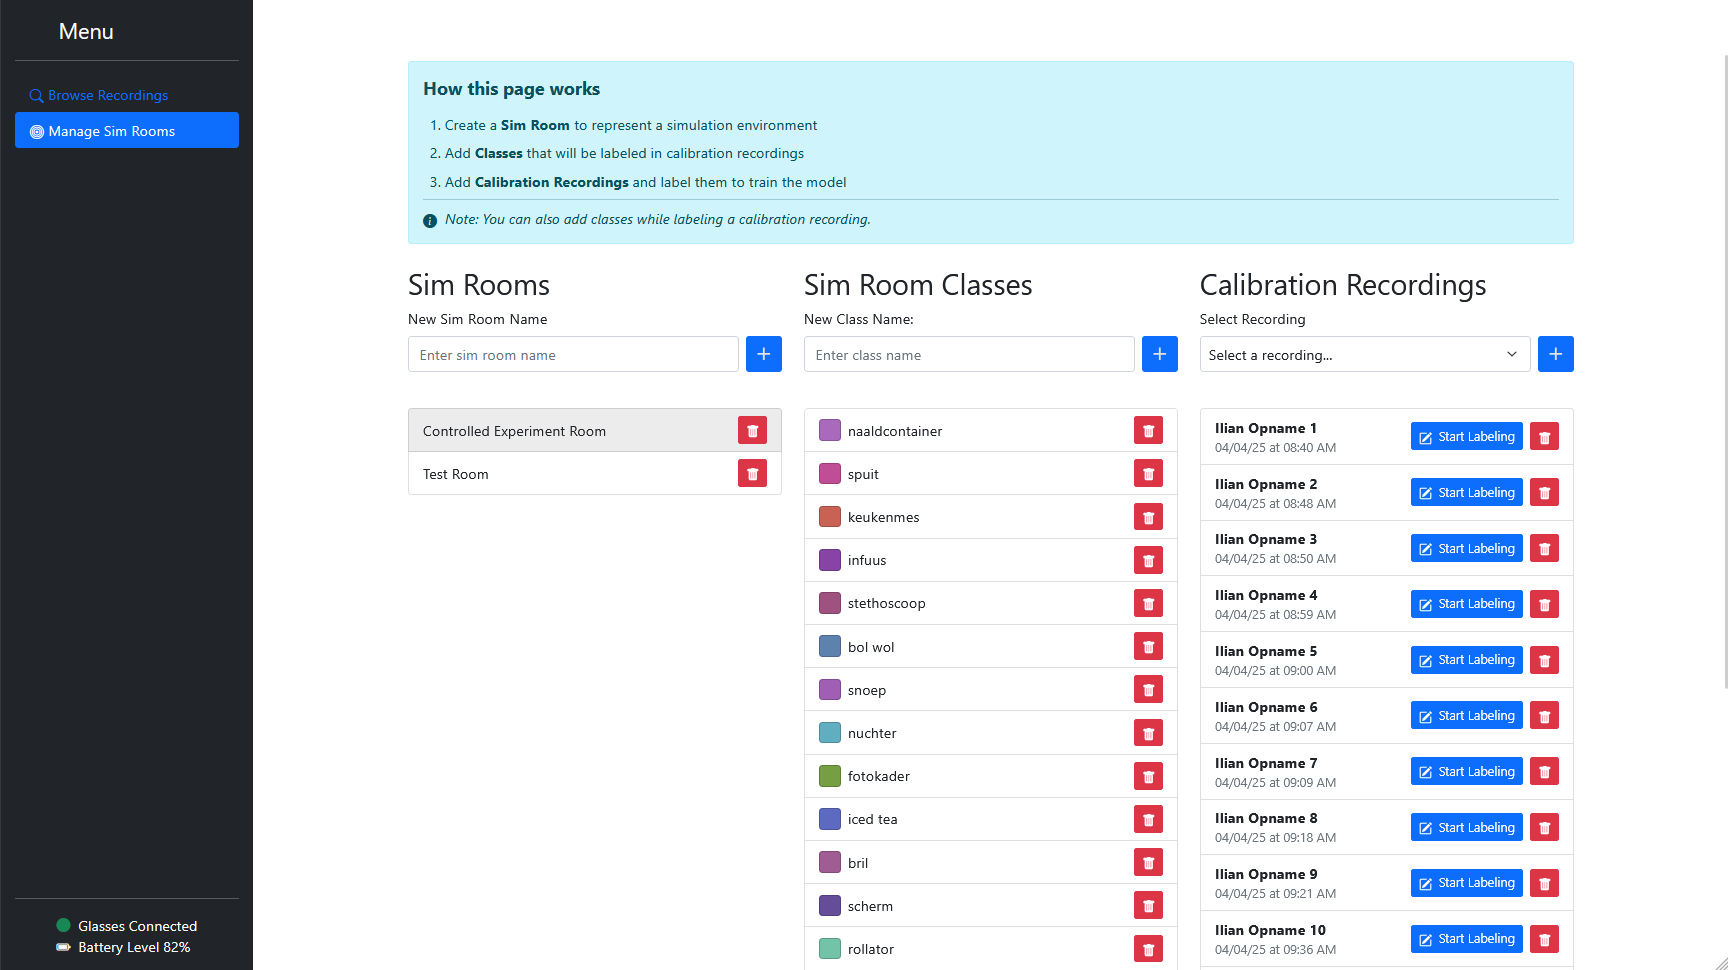
\includegraphics[width=1\textwidth]{simrooms.png}
  \caption[]{\label{fig:simrooms} Voorbeeld van de `Manage Sim Rooms'-pagina waar de simulatieomgevingen kunnen worden gedefinieerd. Hier is de `Controlled Experiment Room' geselecteerd, met een aantal objecten en kalibratie-opnames. }
\end{figure}

In figuur \ref{fig:simrooms} is een voorbeeld te zien van de pagina waar simulatieomgevingen kunnen worden gedefinieerd. 
Deze pagina heeft drie kolommen:
\begin{itemize}
    \item De eerste kolom toont de reeds gedefinieërde simulatieomgevingen, met hun naam, een knop om deze te verwijderen, en een invoerveld om meer simulatieomgevingen toe te voegen.
    \item Wanneer een simulatieomgeving is geselecteerd, worden de bijbehorende objecten getoond in de tweede kolom. Elk object krijgt automatisch een kleur toegewezen die ook gebruikt zal worden in de labeling-tool, en eventueel de visualisatie van de metrieken.
    \item In de derde kolom kan men geïmporteerde opnames selecteren om deze te gebruiken als kalibratie-opnames. Elke kalibratie-opname heeft een knop "Start Labeling". Wanneer men hierop klikt, wordt de labeling-tool geopend met de geselecteerde opname.
\end{itemize}

Merk op dat het mogelijk is om welke opname dan ook te selecteren als kalibratie-opname, waardoor ook praktijkopnames kunnen worden gebruikt!
Zo kunnen we reeds gemaakte opnames van studenten ook gebruiken om de analysemodellen te trainen.
Dit stelt de applicatie eventueel in staat om de opnames te analyseren op basis van manuele annotaties van de trainers.
Deze aanpak zal meer tijd vergen, maar is veel nauwkeuriger dan een automatische analyse. Aangezien het in deze bachelorproef gaat om geautomatiseerde analyse, werd deze optie niet verder uitgewerkt.

Wanneer men een kalibratie-opname verwijdert, heeft dit geen invloed op de opname zelf, maar enkel op de associatie met de simulatieomgeving.
Indien er met de opname werd gelabeld binnen deze simulatieomgeving, worden deze annotaties wel verwijderd. 
Hetzelfde geldt voor de objecten: indien een object wordt verwijderd, worden ook de annotaties die gemaakt werden met dit object in alle kalibratie-opnames verwijderd.

\subsubsection{Labeling Tool}

We hebben het al eerder gehad over de labeling-tool, maar hoe werkt deze nu precies? Dit is één van de belangrijkste onderdelen van de applicatie, en ook het meest complexe.
De labeler kunnen we openen door op de knop "Start Labeling" te klikken van een kalibratie-opname binnen de `Manage Sim Rooms'-pagina.
In de achtergrond worden alle individuele frames uit de opname gehaald en in een map opgeslagen, waardoor het enige tijd kan duren voor de tool opent. De specifieke implementatieredenen hiervoor komen later aan bod.
Het doel van de labeler is om een masker (en een `bounding box') te verkrijgen binnen elke frame van de opname waarin een object zich bevindt.
Natuurlijk zou dit een grote tijdsinvestering vragen bij een volledig manuele tool: Aangezien de framerate van de eyetracker 25FPS is, zou dit betekenen dat we 1500 frames moeten labelen voor een opname van 1 minuut, en dit voor elk object dat we willen labelen.
Het probleem werd opgelost met een semi-automatische labelingtool. Daarbij hoeft men enkel in minder dan tien frames per object te klikken. De tool volgt vervolgens elk object automatisch doorheen de hele opname.
De functies van de labeling-tool worden hieronder verder toegelicht.

\begin{figure}[H]
  \centering
  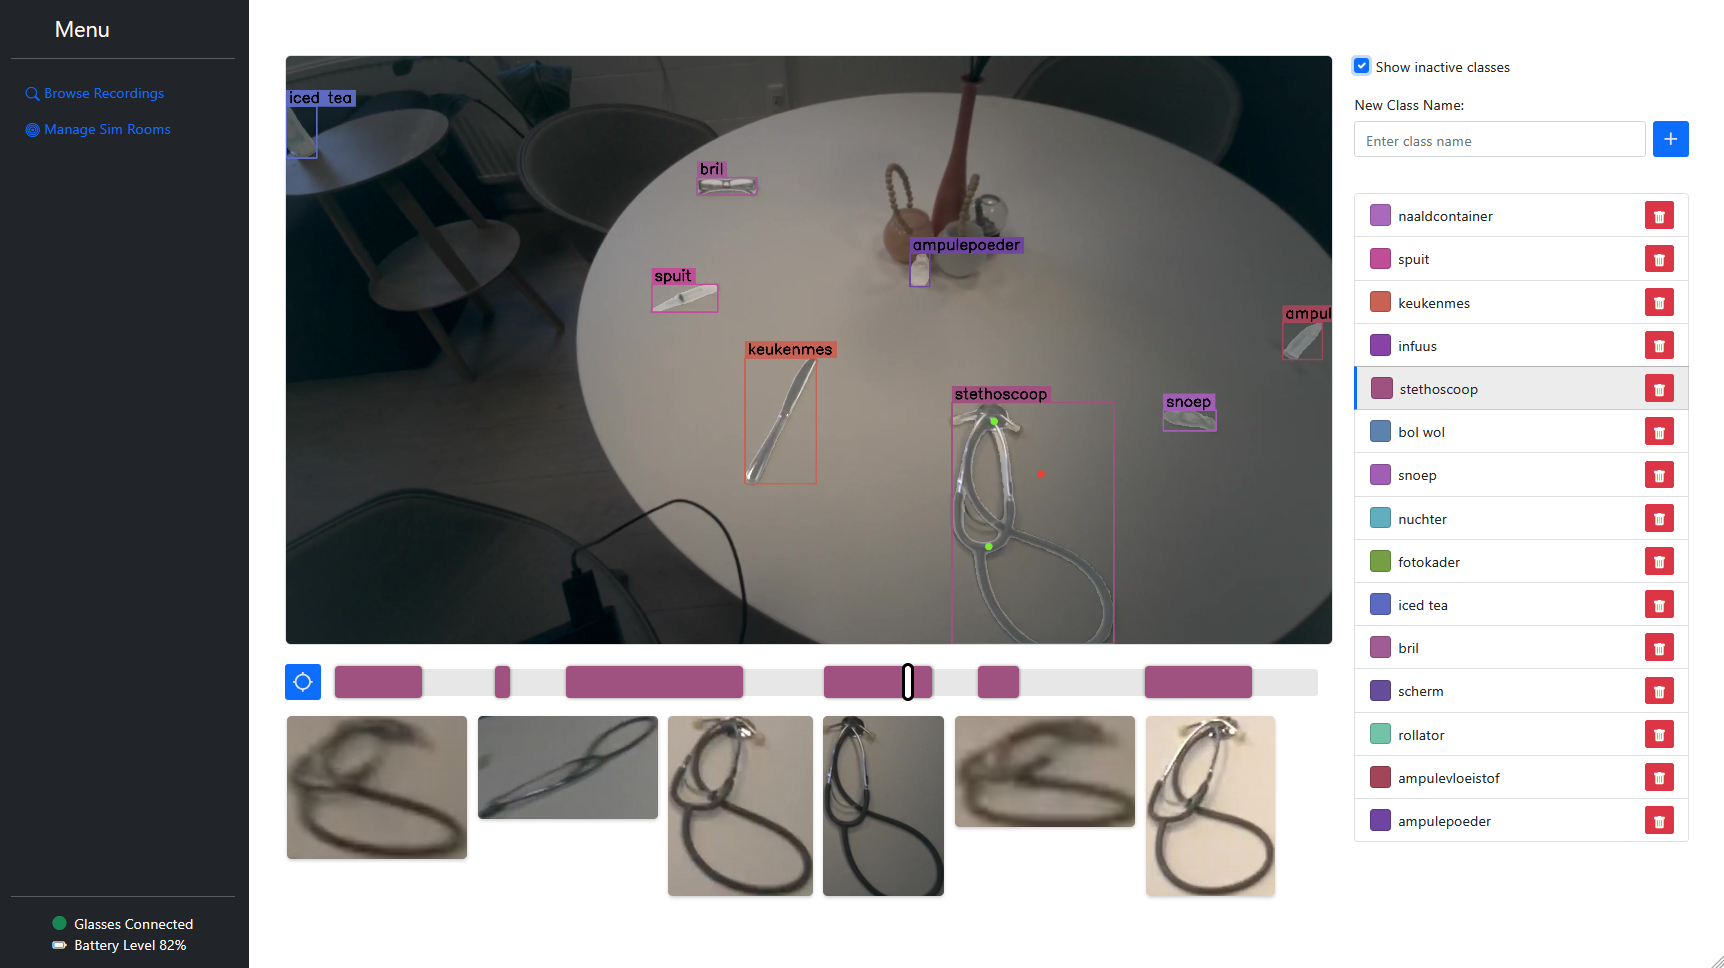
\includegraphics[width=1\textwidth]{labeler.png}
  \caption[]{\label{fig:labeler} Een screenshot van de labeling-tool met vier onderdelen: de labeling-canvas, de tijdlijn, de objectenlijst rechts, en een lijst van gemaakte annotaties onderaan. In dit voorbeeld is het object `Stethoscoop' geselecteerd. }
\end{figure}

Eenmaal de labeling-tool geopend is, zien we een pagina met vier onderdelen (zie figuur \ref{fig:labeler}).
Linksboven zien we het `labeling-canvas', waar de huidige geselecteerde frame van de opname wordt getoond. Onder het canvas is er een tijdlijn die aangeeft waar we ons bevinden in de opname. De tijdlijn markeert ook welke frames het gevolgde object bevatten. 
Binnen deze canvas kunnen we objecten labelen door eerst een object in de lijst rechts te selecteren, en vervolgens te klikken op het canvas.
Hierbij kunnen we een linkermuisklik gebruiken om aan te geven welke delen van de afbeelding deel uitmaken van het object dat we willen labelen (zie de stethoscoop in figuur \ref{fig:labeler}). Met de rechtermuisklik geven we aan welke regio's buiten het object vallen.
Deze zijn respectievelijk gemarkeerd met een groene en een rode stip. Als we met de muis over een stip gaan, wordt deze gemarkeerd. Vervolgens kunnen we erop klikken om de stip te verwijderen.
Na elke muisklik worden het masker en de bijbehorende \textit{bounding box} automatisch geüpdatet om feedback te geven aan de gebruiker.
Onder de tijdlijn zien we een reeks annotaties die we hebben gemaakt, van links naar rechts gesorteerd op tijd. Men kan op deze annotaties klikken om naar de bijbehorende frame te gaan, en ze ook verwijderen door met de muis erover te gaan en op de rode knop te klikken.
Indien men alle stippen verwijdert, wordt de annotatie ook verwijderd.
Eens we tevreden zijn met de annotaties, kunnen we op de blauwe `tracking'-knop klikken aan de linkerkant van de tijdlijn.
Dit start de automatische tracking van het huidige geselecteerde object doorheen de opname, zoals getoond in figuur \ref{fig:labeler-tracking}. 

\begin{figure}[H]
  \centering
  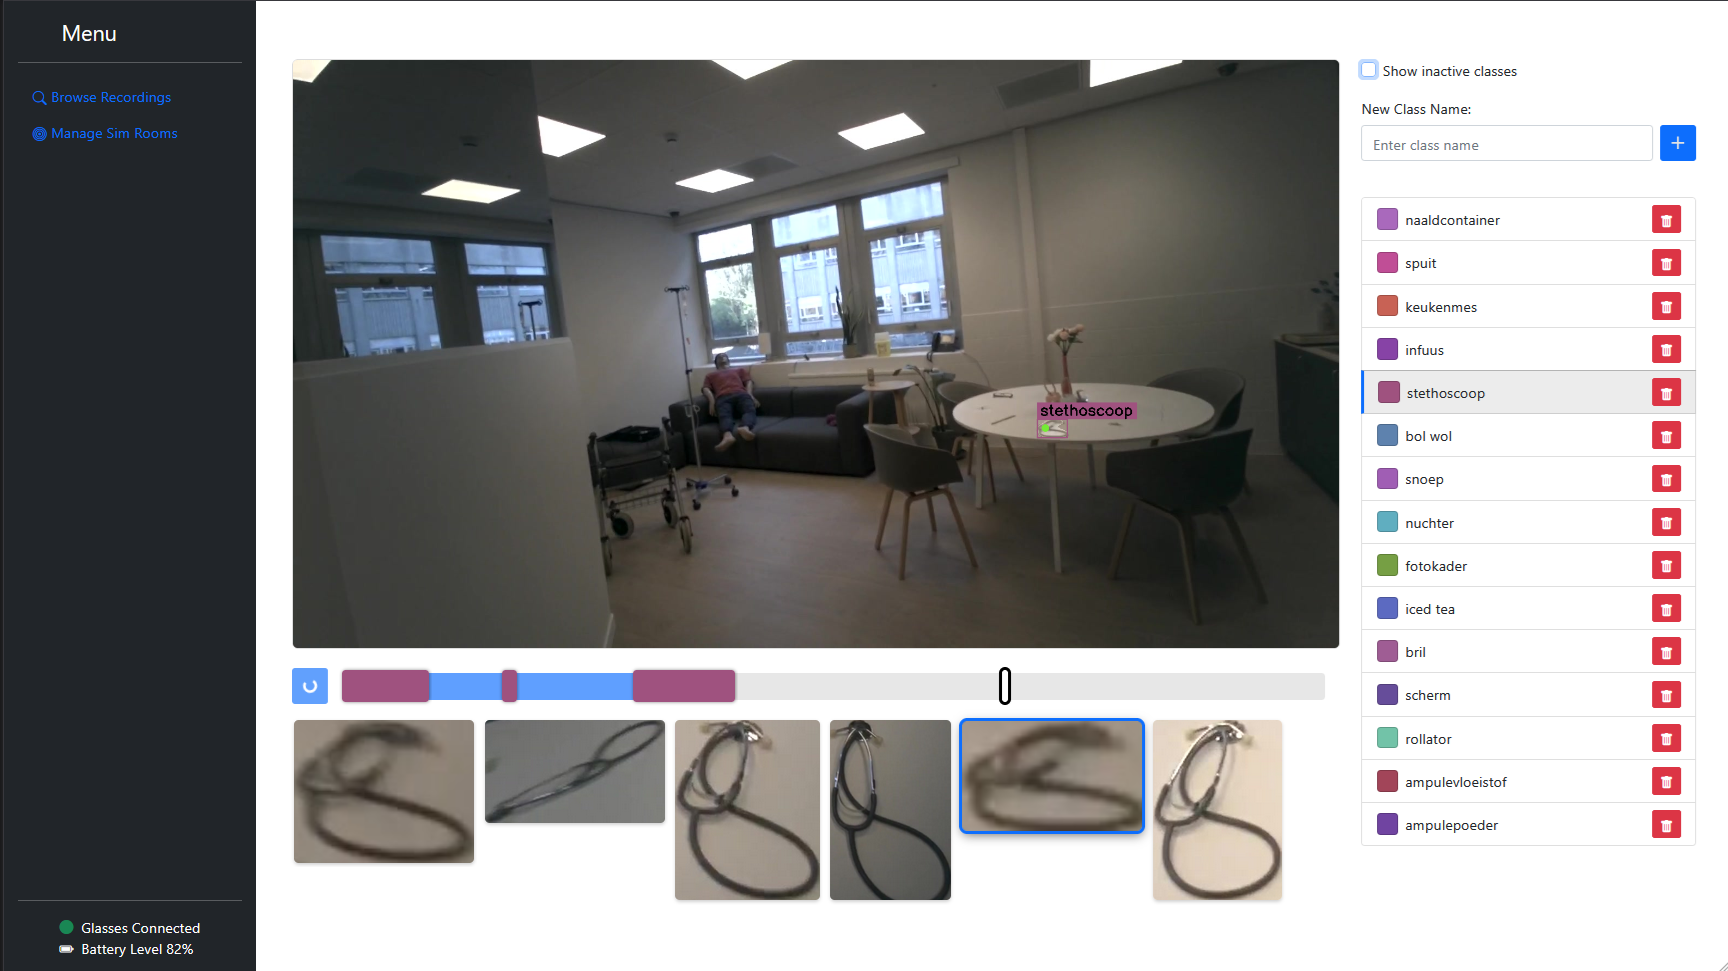
\includegraphics[width=1\textwidth]{labeler-tracking.png}
  \caption[]{\label{fig:labeler-tracking} In deze screenshot zien we dat er een tracking-opdracht gaande is. Hier is ook de optie `Show inactive classes' uitgevinkt, waardoor enkel het actieve object wordt getoond. }
\end{figure}

Om prestatieredenen zullen niet alle frames bekeken worden binnen deze tracking-opdracht. Een annotatie wordt als basis gebruikt voor tracking, en wanneer het object voor een bepaalde tijd uit het beeld verdwijnt, wordt de trackingopdracht stopgezet tenzij er nog annotaties overblijven.
Over het algemeen hebben we slechts één annotatie nodig voor elk gedeelte van de video waarin het object voortdurend in beeld is. Soms zijn echter meerdere annotaties per gedeelte nodig om het trackingresultaat te optimaliseren.
Het specifieke algoritme dat bedacht werd voor de tracking komt aan bod in de technische sectie van dit onderdeel.
Tenslotte bestaat de mogelijkheid dat er veel objecten in beeld zijn waardoor maskers, bounding boxes en labels elkaar overlappen. Om deze reden kunnen we rechtsboven een optie `Show inactive classes', uitvinken om enkel het actieve object te tonen in het canvas.


\subsubsection{Analyse van Eyetracking-Opnames}

Hoewel het aanvankelijk de bedoeling was, werd in de context van deze bachelorproef, geen werkende analyse-tool ontwikkeld maar enkel een proof-of-concept.
De labeling-tool was in dit opzicht de belangrijkste component, omdat deze de annotaties genereert die nodig zijn voor de analyse.
Aangezien de resultaten van de analyses niet betrouwbaar waren, werd hier ook geen pagina voor ontwikkeld.
Indien men in de toekomst een betrouwbaar analysemodel kan ontwikkelen, bestaat de mogelijkheid om een nieuwe pagina te maken die de resultaten van de analyses toont.
Naast de pagina dient dan ook een bijbehorende optie in de navigatiekolom aangemaakt te worden.
De analyses die uitgevoerd werden in deze bachelorproef komen aan bod in Hoofdstuk~\ref{ch:experiment}.

\section{Technische Specificaties}

Voor de ontwikkeling van de applicatie werd een lichtgewicht, modulaire softwarestack gekozen, afgestemd op de specifieke noden van het project. De belangrijkste technologieën en keuzes worden hieronder toegelicht:

\begin{itemize}
    \item \textbf{Backend Framework:} Python met \texttt{FastAPI} werd gekozen omwille van zijn hoge prestaties, asynchrone mogelijkheden (belangrijk voor I/O-intensieve taken zoals data-import en analyse), automatische documentatie en type hinting-integratie.
    \item \textbf{Frontend Aanpak:} In plaats van een zwaar JavaScript-framework, werd geopteerd voor \texttt{HTMX}. Dit laat toe om dynamische interacties te bouwen door HTML direct uit te wisselen met de server, wat de complexiteit van de frontend aanzienlijk reduceert. \texttt{Jinja2} dient als templating engine om deze HTML server-side te genereren.
    \item \textbf{Database:} Een \texttt{SQLite} database werd gebruikt vanwege de eenvoud en het feit dat de applicatie bedoeld is voor lokaal gebruik, waardoor een complexe database server overbodig is. \texttt{SQLAlchemy} werd ingezet als ORM (Object-Relational Mapping) voor een gestructureerde interactie met de database vanuit Python.
    \item \textbf{Hardware Communicatie:} Voor de interactie met de Tobii Pro Glasses 3 werd de officiële \texttt{g3pylib} SDK gebruikt, die toegang biedt tot opnames en statusinformatie via de WiFi-verbinding.
    \item \textbf{Development \& Kwaliteitsborging:} \texttt{Poetry} werd gebruikt voor dependency management. Strikte type hinting met \texttt{Mypy} en code linting/formatting met \texttt{Ruff} dragen bij aan de robuustheid en onderhoudbaarheid van de code. \texttt{Docker} werd ingezet om de applicatie te containeriseren, wat zorgt voor een consistente uitvoeringsomgeving en eenvoudige deployment.
\end{itemize}
Deze keuzes resulteerden in een applicatie die relatief eenvoudig te onderhouden en verder te ontwikkelen is, conform de doelstelling om iteratieve verbeteringen in volgende bachelorproeven mogelijk te maken.

\subsection{Softwarearchitectuur}

\subsection{Labeling Tool}